\chapter{Application architecture}
\label{sec:application-architecture}

    This chapter covers the application architecture. We present here the essential services and application components that enact the current and the new life-cycle processes.

	\section{Prototypical application structure}
	
	This section presents the application architecture from the solution architecture point of view. A generic solution architecture is depicted in Figure \ref{fig:application-view}.
	
	The application architecture presented covers the application as a ``white box'', its internal component structure, services and interfaces with adjacent applications. Typically the solutions architecture takes the technology aspects into account, accounting for parts of the infrastructure.
	
    \begin{figure}[h]
		\centering
		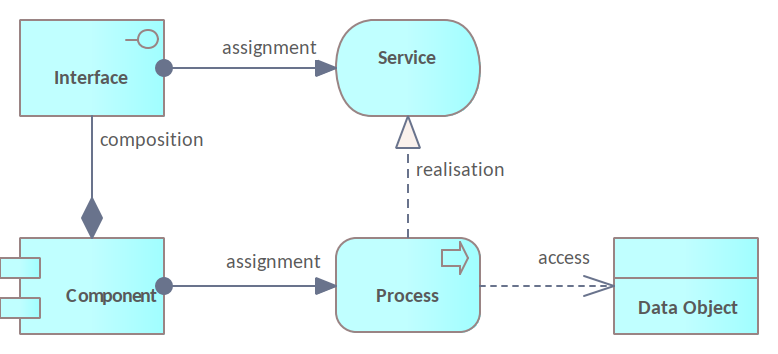
\includegraphics[width=.6\textwidth]{images/views/Application view.png}
		\caption{The prototypical application structure view}
		\label{fig:application-view}
	\end{figure}

	The central element of the application architecture is the \textit{application service}, which represents application behaviour or functionality. The application services, from an inter-layer perspective, serve the processes in the business layer and provide support for their realisation. 
	
	The application services are realised through application processes. The processes have application components assigned to them signifying their place of encapsulation. Application components are modular and replaceable blocks encapsulating implementation of application services and functionalities. In practice, for clarity, we take a shortcut, and say that the application services are realised through \textit{application components} directly.
	
	Components are said to expose interaction \textit{interfaces} which are modelled, in ArchiMate, as proper parts of the components. The interfaces are assigned to services signifying how the latter are to be accessed and consumed. 
	
	Also, components, as well as processes they encapsulate, access \textit{data objects}, which are passive components of the application architecture.

	The solution architecture presented in this section is an adaptation of the generic architecture. Here we focus on presenting what application services are used to support each business process. Moreover, we are interested in grasping the difference in the application layer, between the current and new versions of the business processes. 
	
	To do so, we split the application view diagrams into three vertical lanes. The left lane hosts the current version of the business process as well as the application services and components that are used to support it. In the right lane, we place the new business process and the new application services and components that will have to be adopted for the digital transformation. The middle lane hosts the services and components that are are currently employed and will be carried over into the new application architecture: they are common to both the current and new architectures.

	Below we present an overview of the application architecture, in terms of services alone, depicting how the asset life-cycle stages are served.
	
	\section{Current and new application service architecture}
	\label{sec:application-overview}
	
	This section presents how the asset life-cycle stages are supported by the application services. The current application architecture is depicted in Figure \ref{fig:application-current} and the new one in Figure \ref{fig:application-new}. The services employed in each of the architectures are mostly the same, with a few exceptions. What differs more significantly is their utilisation in the asset life-cycle stages. For this reason, we set them side-by-side to provide a contrasting image. 
	
	\begin{figure}[h]
		\centering
		\begin{minipage}{0.485\textwidth}
			\centering
			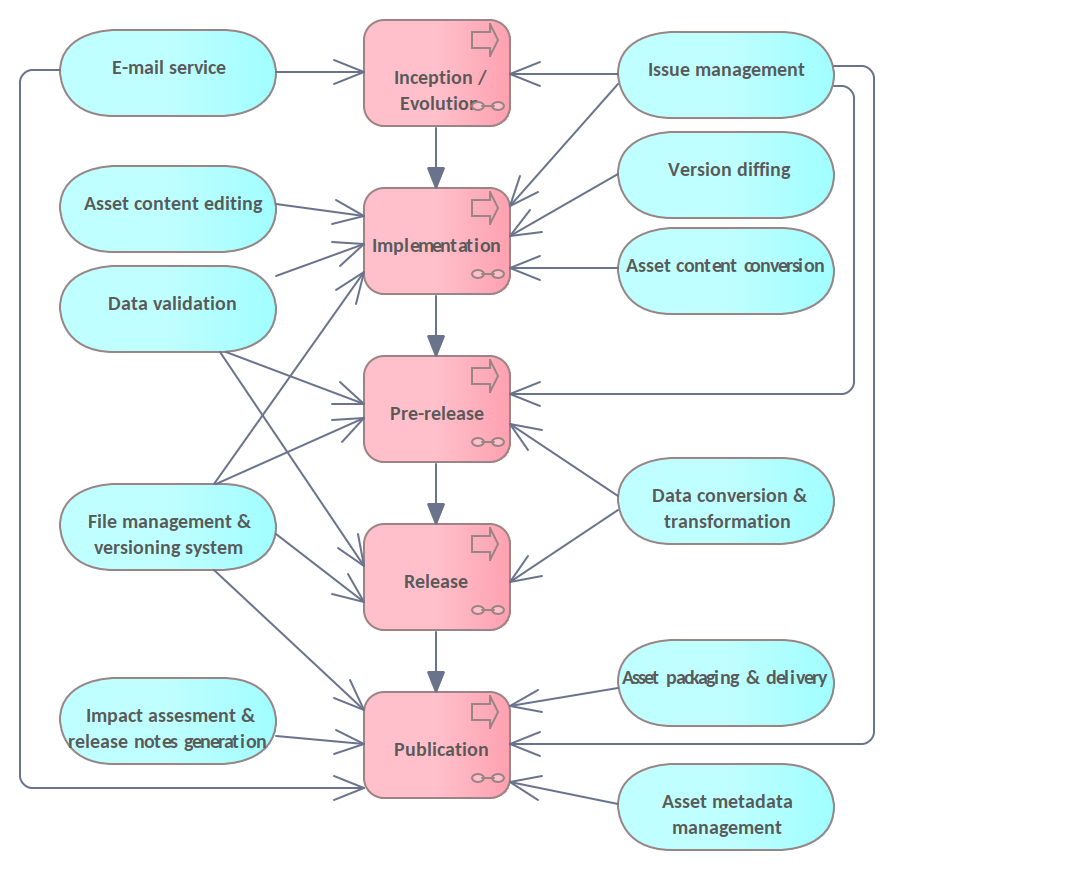
\includegraphics[width=1.3\textwidth]{images/application/Application Services (current).png}
			\caption{The application services that serve the current asset lifecycle}
			\label{fig:application-current}
		\end{minipage}\hfill
		\begin{minipage}{0.485\textwidth}
			\centering
			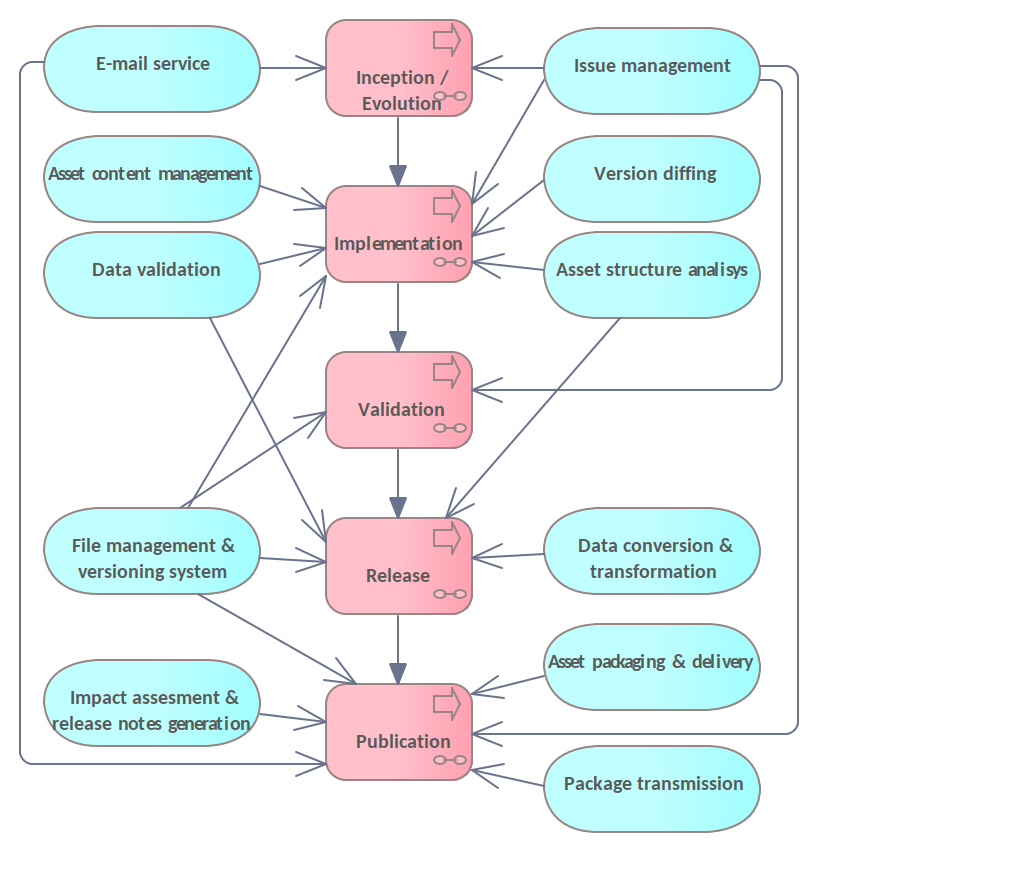
\includegraphics[width=1.3\textwidth]{images/application/Application Services (new).png}
			\caption{The application services that serve the new asset lifecycle}
			\label{fig:application-new}
		\end{minipage}
	\end{figure}
	
%	\begin{figure}[h]
%		\centering
%		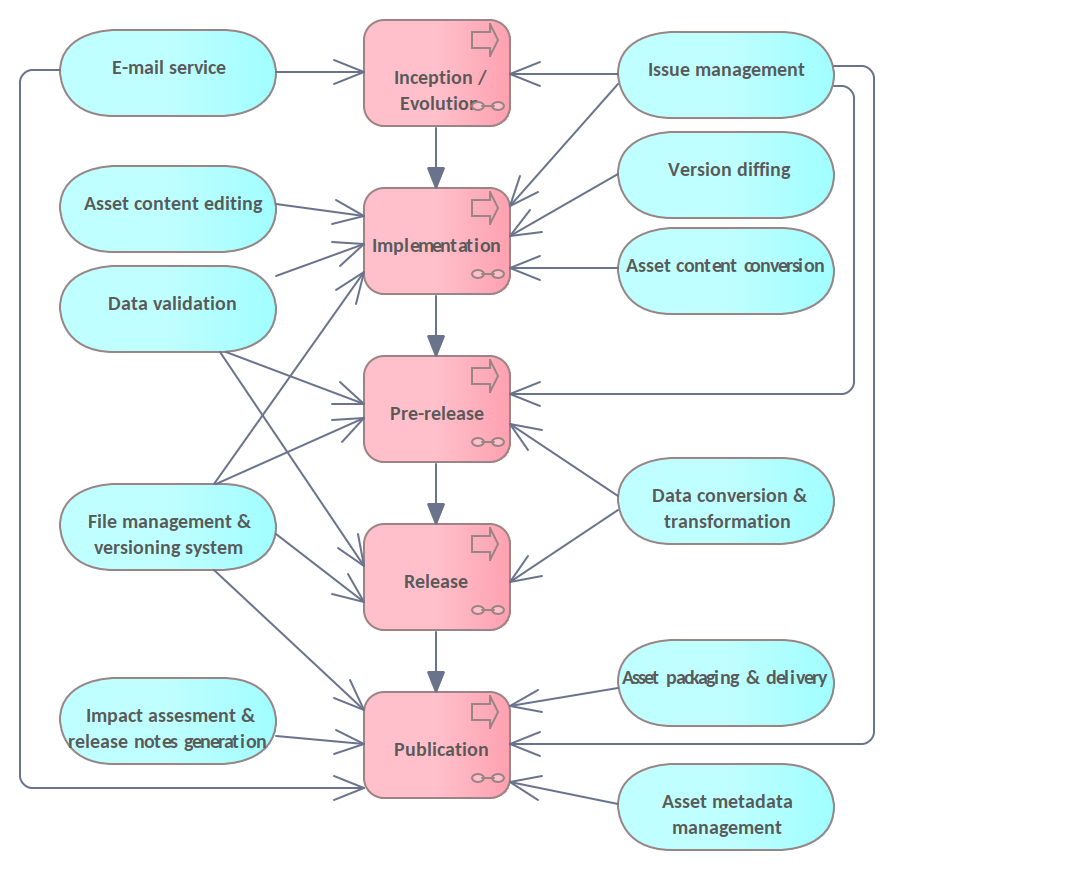
\includegraphics[width=.75\textwidth]{images/application/Application Services (current).png}
%		\caption{The application services that serve the current asset lifecycle}
%		\label{fig:application-current}
%	\end{figure}

	We start the description from the top of the diagram following the sequence of process stages. First is the \textit{e-mail service}. It represents the entire set of capabilities for sending emails covering both the email server and email client. This is realised via the Outlook system \citep{outlook}. 
	
	The \textit{issue management} service represents the capability of recording, documenting and analysing a change request case in a distributed collaborative manner between multiple roles and actors. This is realised via the Jira system \citep{jira}. 
	
	\textit{Asset content editing} is the service which enables the documentalists in the team to modify asset content and hence implement the request cases. This service is realised by MS Excel desktop software \citep{excel}.
	
	The \textit{asset content conversion} service implements the conversion between MS Excel workbook and CAT-XML forms of the asset content. The two representations are equally expressive and the conversion process runs in both directions $ Excel \rightarrow XML $ and $XML \rightarrow Excel $.
	
	\textit{Version diffing} is a service which calculates and presents the difference between two versions of the same asset. The \textit{data validation} service is self-explanatory. It checks whether the asset content is correct, or not. The asset content conversion, version diffing and data validation services are realised by components that comprise the legacy workflow, which is currently in use.
	
	\textit{Asset document management} provides capabilities for describing, storing and producing documents about assets in various human-readable formats (e.g. HTML, PDF, docx). It also allows for document metadata management. Currently, this capability is realised by PDF forms, called Asses Description Document (ADD), which are produced from XML-DITA sources \citep{dita-day2005introduction, dita-spec} using Adobe FrameMaker \citep{framemaker}. 
	
	\textit{Asset metadata \& workflow management} is a service which centralises the flow of the automated processes. It is currently realised by legacy workflow implementation. 
	
	The \textit{file management \& versioning} service enables storing the content and and tracing the evolution of assets. This service is realised by the SVN system \cite{svn}.
	
	The \textit{data transformation} service stands for a generic capability of transforming data from one form and format into another. The main transformation flow is from RDF data source into representations that are already supported by the current workflow. Currently, this service is realised by a multitude of custom-built transformation procedures, some of which are chained to produce the desired outcome. This service is realised by components that are part of the legacy system. 
	
	The \textit{asset packaging} service prepares assets for transmission to the dissemination systems, specifically Cellar. It covers functionalities including assembling the necessary asset representations together with their documentation, generating necessary technical metadata and zipping the assets in a manner that is acceptable for partner dissemination systems. The type of package and the asset metadata description varies, yet among the most prominent ones are METS \citep{mets}, IMMC\footnote{see \url{https://op.europa.eu/en/web/eu-vocabularies/immc}} and DCAT \cite{dcat2}.
	
	\enlargethispage{1em}
	
	The last service to mention that is employed in the current life-cycle process is the \textit{impact assessment \& release note generation} service. Its title is again self-explanatory. The values it provides are the release notes that are published with assets and describe the list of changes implemented in each version. The impact assessment is a type of report which includes assessments for target stakeholders which usually are service provides whose systems depend on the assets published by the SU. These special impact assessments may target whether a given aspect of an asset has changed which may disrupt functioning systems. So, a series of specific checkers and reports are produced to safeguard the partners. 
	
	The new application architecture (Figure \ref{fig:application-new}), as mentioned above, re-configures how services are used across process stages. It replaces the asset content editing service by a new one which is \textit{asset content management}. This service is realised by a fully-fledged semantic web editing system -- VocBench3 \citep{stellatovocbench}. In addition, two more services are added: asset structure analysis and package transmission services.
	
	The \textit{asset structure analysis} implements an automatic fingerprinting of the asset structure which provides an insight into how the managed asset is realised and substantiated. This fingerprinting serves as an indicator for the structural validation in the implementation step. For example, a missing or extra property will be spotted with this service. 
	
	The \textit{package transmission} provides the possibility to automatically deliver and ingest the prepared packages into the dissemination system, rather than the publication officer having to perform this operation manually. 
	
%	\section{New application service architecture}
%	\label{sec:application-new}	

%	\begin{figure}[h]
%		\centering
%		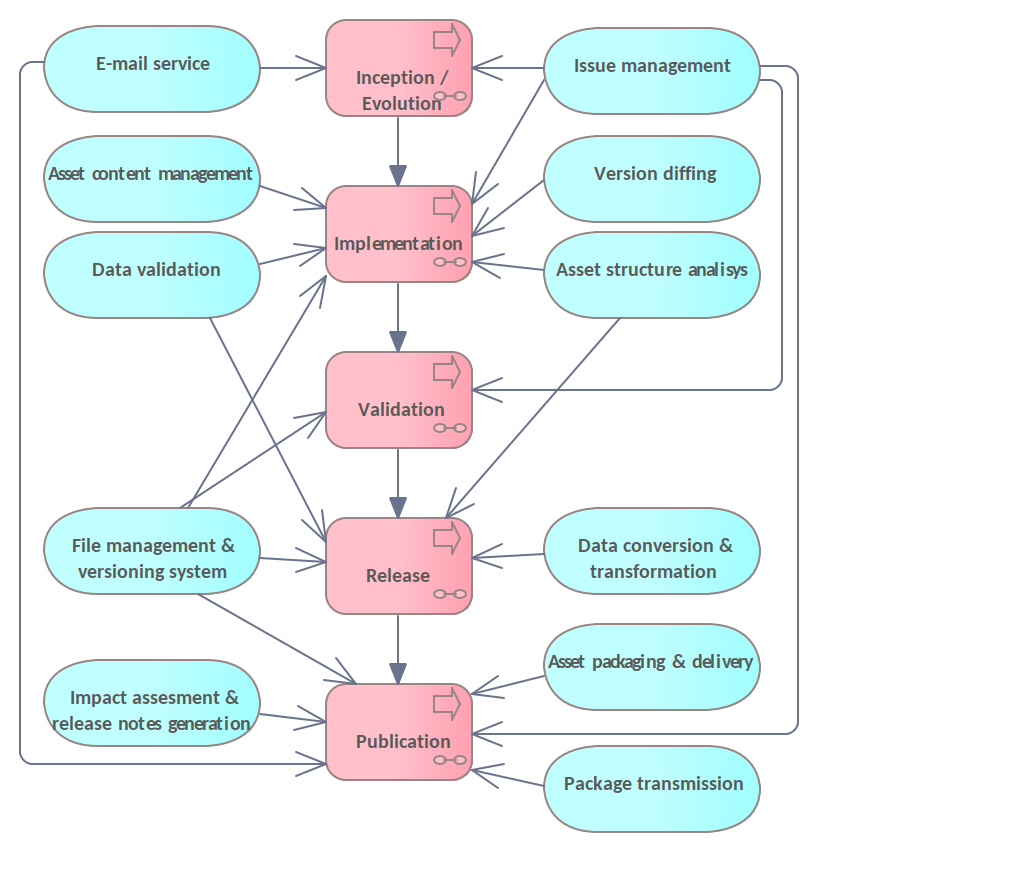
\includegraphics[width=.75\textwidth]{images/application/Application Services (new).png}
%		\caption{The application services that serve the new asset lifecycle}
%		\label{fig:application-new}
%	\end{figure}	
	
	\section{Inception \& evolution stage services and components}
	\label{sec:evolution-application}
	
	In the first stage of the asset life-cycle, the technical requirements are limited to client communication and the request documentation services as depicted in \mbox{Figure \ref{fig:application-inception-evolution}}. The diagram is split into three lanes. The right lane accounts for the new components, while the left line for the current ones. The components that are common to both are situated in the middle lane. 

	\begin{figure}[h]
		\centering
		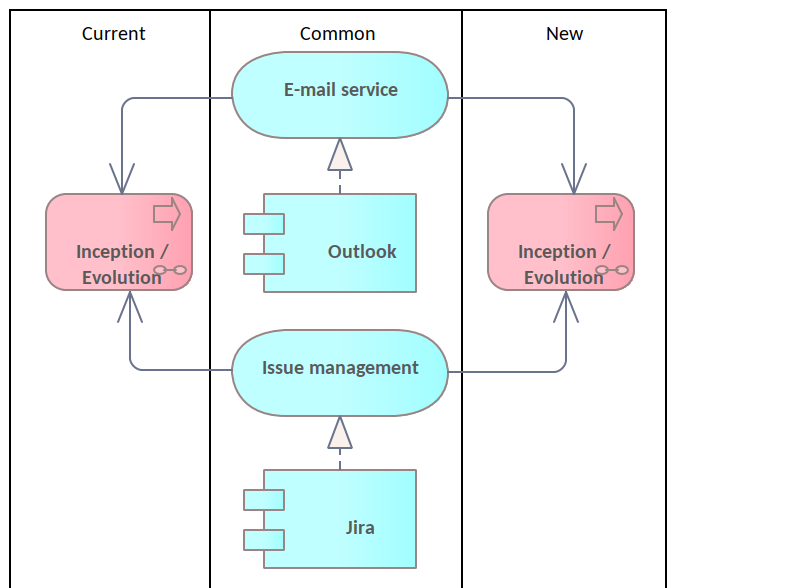
\includegraphics[width=.6\textwidth]{images/application/InceptionEvolution.png}
		\caption{The application services and components that serve the current and new inception and evolution stage}
		\label{fig:application-inception-evolution}
	\end{figure}
	
	The life-cycle stages are represented as red rectangles situated in the left and the right lanes. In the middle lane are the email and issue management services because they are involved in both the new and current architectures. 
	
	The email service is realised by the Outlook software. Issue management is realised by the Jira system. No changes are foreseen in the way these services are realised in the future. 

	\section{Implementation stage services and components}
	\label{sec:implementation-application}	
	
	The implementation stage is the first place where considerable differences are visible in the way the application architecture is organised. This is depicted in Figure \ref{fig:application-implementation}.
	
	\begin{figure}[!h]
		\centering
		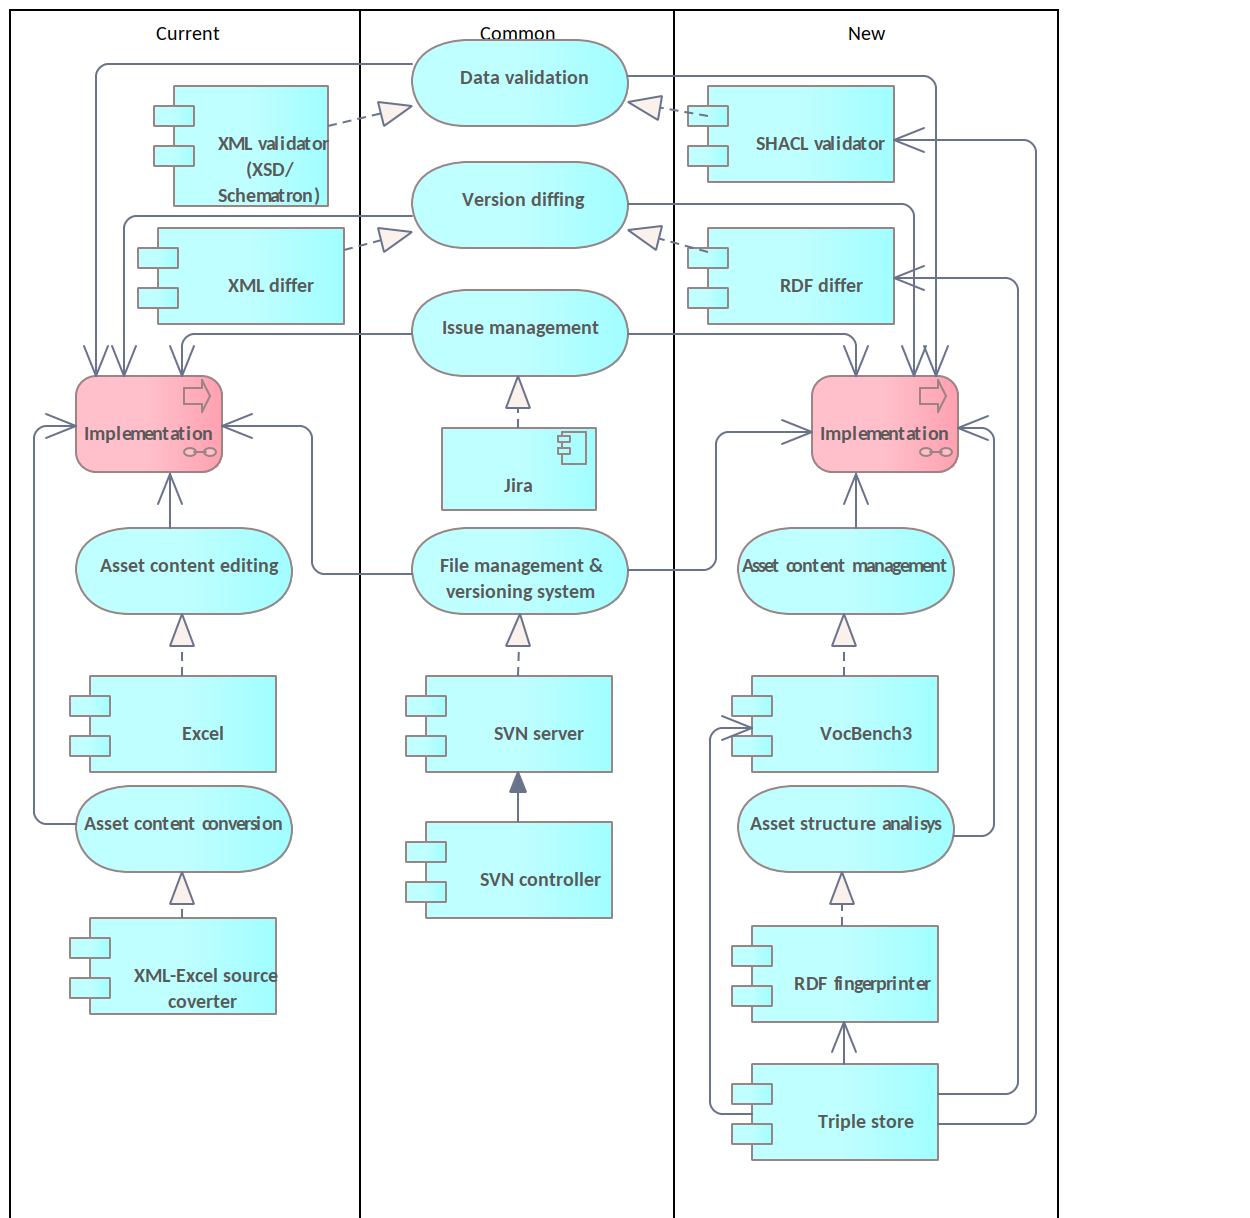
\includegraphics[width=.9\textwidth]{images/application/Implementation v3.png}
		\caption{The application services and components that serve the current and new implementation stage}
		\label{fig:application-implementation}
	\end{figure}
	
	This section presents the common services first, situated in the middle lane of the diagram, and then the particularities which are situated at the left and right sides of the diagram are presented. 
	
	The issue management system is involved and is realised the same way as in the inception/evolution stage (Section \ref{sec:evolution-application}). In the following sections the services and their realisation that have been already discussed will no longer be addressed.  
	
	File management \& versioning is realised through SVN \cite{svn}. In the current application architecture this serves as a foundation for process automation, the triggers being any operations within the SVN repository. The mechanisms employed are similar to what an automation server is doing in the software development context: triggering automatic building, testing and deploying, facilitating continuous integration and continuous delivery. No such automation server is, however, used due to infrastructure limitations that existed in the past and a custom SVN handler component was developed within the legacy workflow system. 
	
	In the new architecture, the possibility to continue the same practice of automating process executions based on SVN triggers is still there. Moreover, it is advisable replacing the current SVN handler by an automation system, such as Jenkins \citep{jenkins} or Bamboo \cite{bamboo}. This suggestion is not depicted in the diagram because the current workflow SVN handler could still serve in the immediate future; however, in the long run, the alternative is recommended.
	
	In the current system, the asset metadata and workflow design management is centralised in a custom-built XML file called the ``Vocabulary table''. The vocabulary table is an XML file which serves three functions. It contains descriptions of currently-administered digital assets, descriptions of generic process execution flows and decision rules for alternative flows specific to some assets. This aggregation of multiple responsibilities complicates both the maintenance and evolution and shall be separated in the future. 
	
	Operationally, the vocabulary table is used by the legacy system for deciding what chains of operations shall be executed start to end, without the possibility to monitor or manage the process steps. It is also becoming increasingly difficult to maintain, adapt and extend workflow descriptions indicated in the vocabulary table. This challenge can be overcome by adopting a modern workflow management system. 
	
	% rephrase
	%For this reason, we say the it is ``workflow design management'' and not the actual ``workflow management'',  because we deal here with description and configuration of the execution paths and decision rules (plus asset metadata) which are enacted by the legacy workflow system. This aggregation of the two responsibilities complicates both the maintenance and evolution both shall be separated in the future.  
	
	Later, after adoption of the digital transformation proposed in this architecture, the asset metadata and workflow design management service need to be broken down into two parts: asset metadata management and workflow management. The metadata management can be realised through a DCAT \citep{dcat2} cataloguing software. 
	
	Workflow management could be taken over by any workflow management and execution engine that implements service orchestration\footnote{In system administration, orchestration is the automated configuration, coordination, and management of computer systems and software. A number of tools exist for automation of server configuration and management, including Ansible, Puppet, Salt, Terraform, and AWS CloudFormation.} or choreography\footnote{Service choreography is a form of service composition in which the interaction protocol between several partner services is defined from a global perspective.}. 
	
	This could be taken one step further towards a BPMN \citep{bpmn-introduction} execution engine such as Camunda BPM, Flowable and Bonita BPM. There is an installation and configuration overhead for such a system, but the investment is worth considering knowing that they ship with tools for creating workflow and decision models, operating deployed models in production, and allowing users to execute workflow tasks assigned to them. 
	
	Now we should focus on the top of the middle lane, to the data validation and version diffing services. The components that realise them are split between the left and right lanes. This means that currently validation is performed using the XML validator and the version diffing is performed using XML differ, while in the new application, validation is realised using a SHACL \citep{shacl-spec} validator, and version diffing using an RDF differ. The SHACL validator and RDF differ are custom components developed for the new application context.
	
	In the right lane, the asset content editing and the asset content conversion services were introduced in Section \ref{sec:application-overview}. They are the gateway for the asset authoring officers to implement change request cases. Content editing is realised through MS Excel running on the documentalists' workstations. Once the edit is finished, the updates are committed to the common SVN repository. The changes are picked up by the SVN handler in the legacy workflow system and trigger a conversion process from MS Excel to XML, and then back to MS Excel. The conversion is realised by another legacy component implemented to do exactly that. The resulted conversion is committed into the SVN repository again. This circular conversion, as explained in Section \ref{sec:implementation-current}, is necessary because the main source of the assets is represented as CAT-XML, whereas MS Excel workbook is merely an extension that enables user-friendly editing capabilities.
	
	In the new version of the implementation stage, the main source of the assets is represented as SRC-AP \cite{src-ap-vb3}, a particular form of SKOS \citep{skos-spec} and is serialised as RDF \citep{rdf11}. The editing is covered by the asset content management service, which is realised by the VocBench3 system \citep{stellatovocbench}. When the authoring officer finishes the implementation of a request case, the content is exported from VocBench3 and committed into the SVN common repository. This commit triggers automatic SHACL validation, RDF diffing and structure analysis operations, which write the results back into the common repository for the editor to look at and verify the implementation correctness. 
	
	Asset structure analysis service is realised by the RDF fingerprinter component which is necessary for the quality assessment in this and the next stage of the asset life-cycle. Finally, asset documentation management service was described in \mbox{Section \ref{sec:application-overview}.}
	
	The new RDF-based components rely mostly on the existence of an RDF triple store service, which is a database ensuring persistence, accessibility and data query. This triple store component is depicted not as realising any service in particular, but as serving other components: RDF fingerprinter, SHACL validator, RDF differ and VocBench3, so that they function as expected this way, creating a dependency between them. We use a generic label ``triple store'' here to express that it is of little importance what system is chosen in particular. Among the candidates we can mention are Fuseki, Virtuoso, GraphDB, StarDog, AnzoGraph,... the list can continue. 
	
	This brings us to the end of the implementation stage description which provided us with a parallel between the services and components as they are used currently and how the new application should be implemented. 
	
	\section{Pre-release \& validation stage services and components}
	\label{sec:validation-application}
	
	The stages following the implementation in both the current and new life-cycle processes differ. In Section \ref{sec:lifecycle-new} was described that the current life-cycle includes the pre-release stage, while in the new life-cycle replaces it with a stage called ``validation stage''. This is reflected in the application architecture as well and depicted in Figure \ref{fig:application-validation}.
	
	\begin{figure}[h]
		\centering
		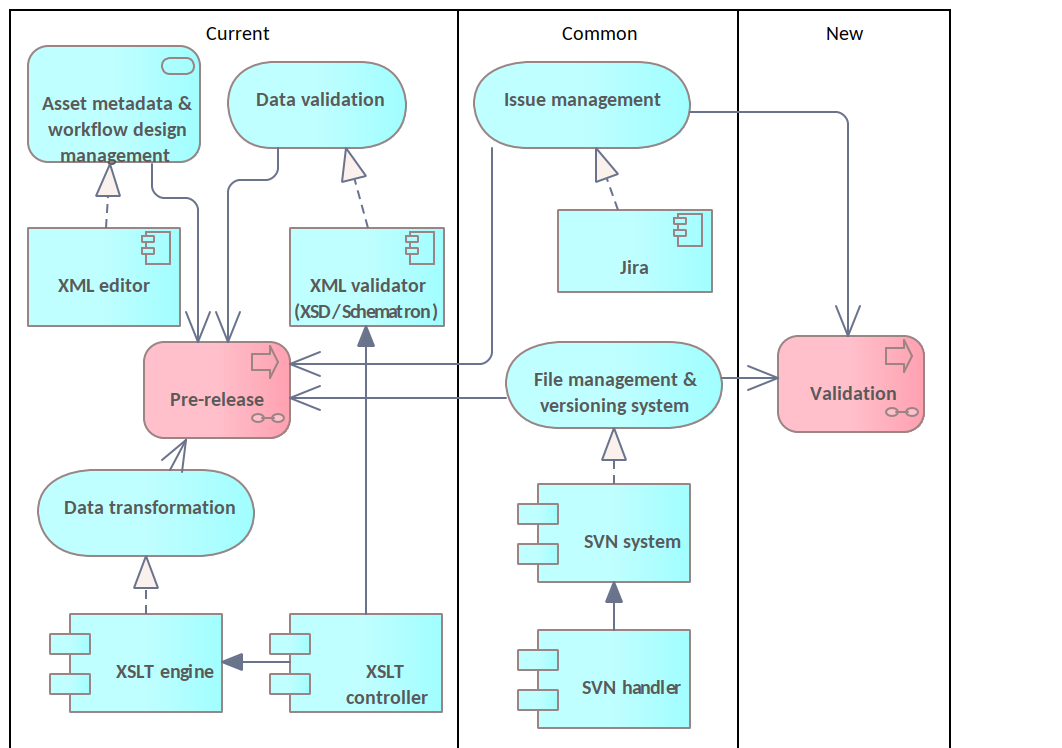
\includegraphics[width=.9\textwidth]{images/application/Validation & Pre-release v3.png}
		\caption{The application services and components that serve the current pre-release and the new validation stages}
		\label{fig:application-validation}
	\end{figure}
	
	The current pre-release stage, on the left lane of the diagram, involves asset metadata and workflow design management service, described in Section \ref{sec:implementation-application}, due to the workflow automation involved in this stage. 
	
	The data validation was also described in Section \ref{sec:implementation-application}. One thing that was not mentioned is that the validation relies on an XSLT \citep{xslt3-Kay} controller component which triggers the XML validator component, also the XSLT transformation component realising the data transformation service.
	
	The data transformation service is used currently in the pre-release stage to format the RDF/XML content. Internally, this operation is known as SKOS ``prettification'', i.e. making the SKOS-RDF/XML easier to work with. This operation will no longer be necessary in the new architecture and the XSLT transformation component will only be employed in the next stage: release.
	
	The issue management, file management and versioning services are used in the pre-release stage and are the only ones necessary in the validation stage. Therefore, they are placed in the middle, common, lane. These services have been detailed in Section \ref{sec:evolution-application} and \ref{sec:implementation-application}. The validation stage requires nothing more than these because it is mostly a manual process executed by the validation officer who checks the validation artefacts generated previously in the implementation stage, as explained in Section \ref{sec:validation-new}.	

	\section{Release stage services and components}
	\label{sec:release-application}	
	
	The release stage is significantly unbalanced in terms of the services employed currently and what is foreseen in the new architecture: this is reflected in the application architecture depicted in Figure \ref{fig:application-release}. 
	
	\begin{figure}[h]
		\centering
		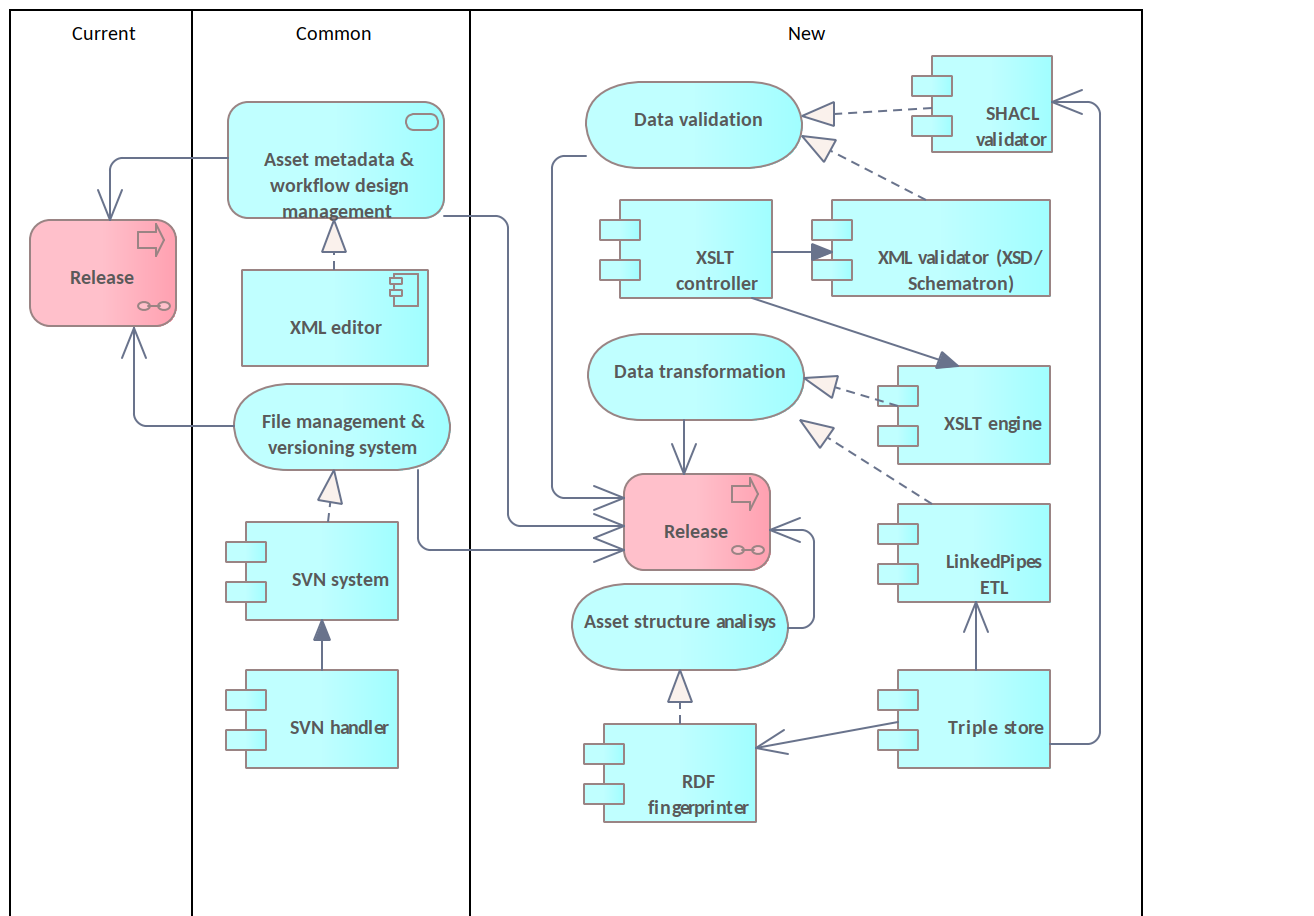
\includegraphics[width=.9\textwidth]{images/application/Release v3.png}
		\caption{The application services and components that serve the current and new release stage}
		\label{fig:application-release}
	\end{figure}

    \enlargethispage{3em}
    
	Currently, in the release stage described in Section \ref{sec:release-current}, the asset(s) are mainly copied from one part of the common repository into a another which is dedicated to the artefacts that follow to be published. 
	
	
	
	In the new release stage, in addition to the copying operation, all data transformation operations described in Section \ref{sec:publication-current} are also executed leaving the (new) publication stage to deal with packaging and dissemination mainly (from a technical perspective).
	
	This is reflected in the new application architecture depicted in the right lane. The data transformation services are employed here, not only in their current form, dealing with various formats consumed by the current clients (XSD, MarkXML, GeoJSON, etc.), but also with complex transformation operations on RDF representation. The former is realised through the same XSLT engine component, while the latter is realised through a new component called LinkedPipes ETL \citep{linkedpipes-klimek2016linkedpipes,linkedpipes-klimek2017linkedpipes}.
	
	The situation is similar with the data validation service: both the current validation component based on XSD schemas and Schematron checks, and a new validation based on SHACL shape checks, are necessary. Both validation types are used because current data formats and new data formats needs to be formally verified before being published. This validation, however, aims to ensure primarily that the transformation processes run correctly and, to a lesser effect, the content correctness which is already assessed in the previous validation stage. The asset structure analysis service was addressed in Section \ref{sec:implementation-new}. Also, the new components that operate with RDF data require a triple store which is depicted in the left lane as serving the depending components.
	
	
	\section{Publication services and components}
	\label{sec:publication-application}	
	
	The publication stage is the last one in the asset life-cycle process. Its application architecture is depicted in Figure \ref{fig:application-publication}. There is not much difference between the two, most services and components being placed in the middle lane, common to both. 
	
	\begin{figure}[!h]
		\centering
		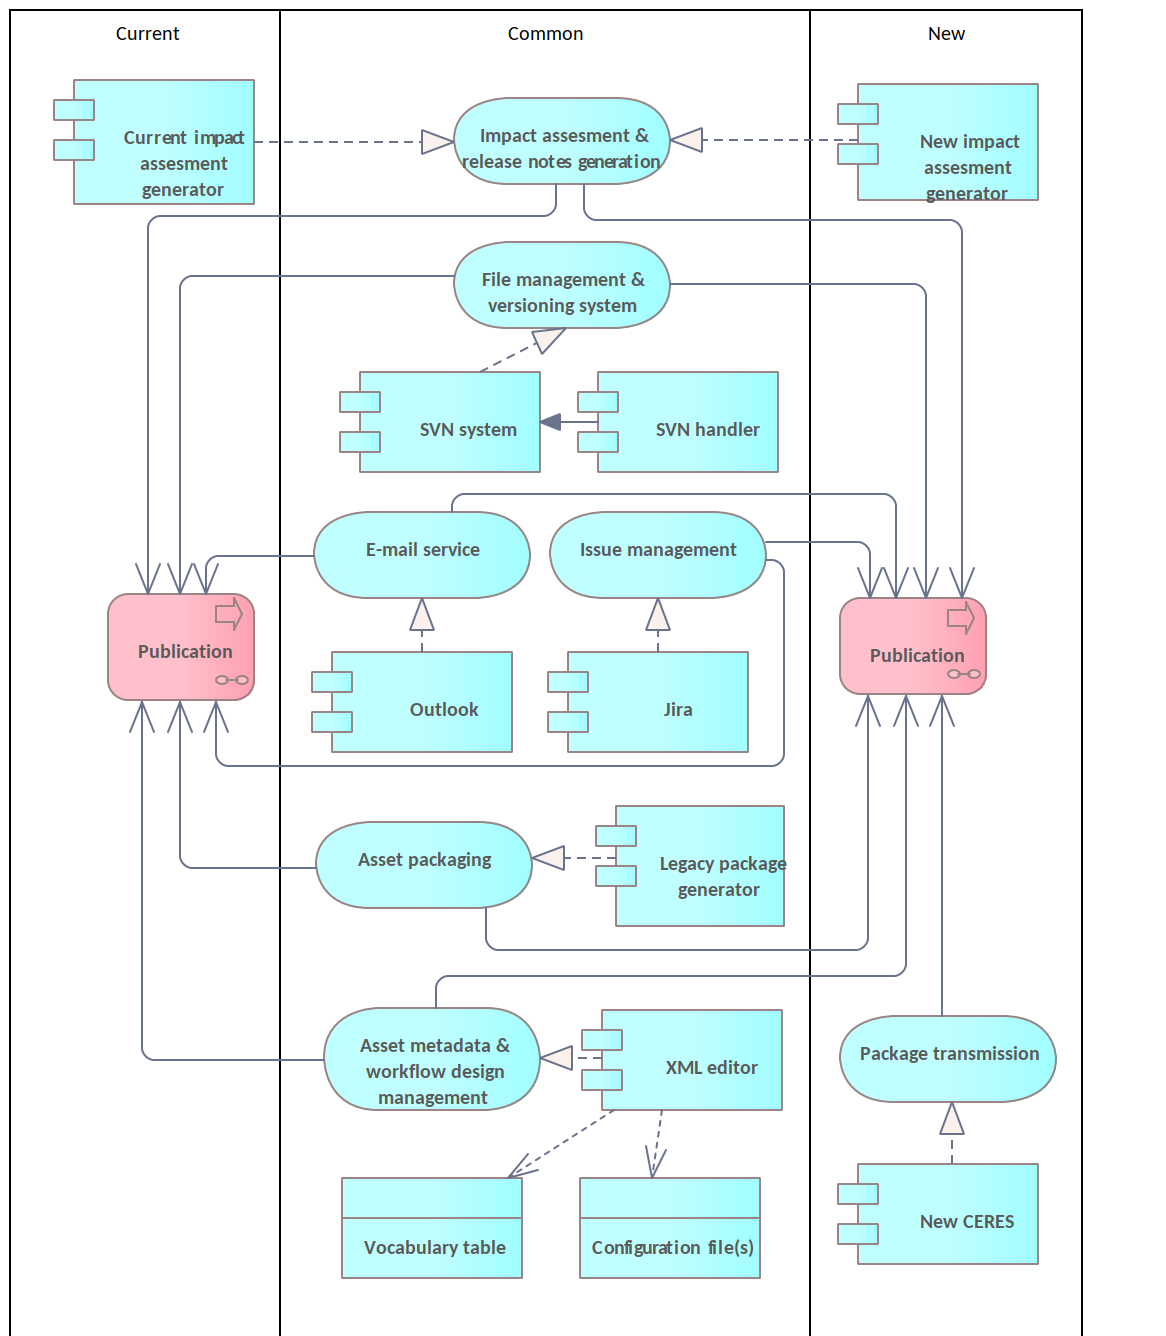
\includegraphics[width=.9\textwidth]{images/application/Publication v3.png}
		\caption{The application services and components that serve the current and new publication stage}
		\label{fig:application-publication}
	\end{figure}

	New and specific to the publication stage is the impact assessment. The release notes generation service provides the basic communication artefacts about what has changed between two versions of an artefact and what is contained in a publication. To a large extent, it is based on the diffs generated in the implementation stage, but not limited to those. However, this has an impact on how the component functions because the diffs of two XML files are different from the diffs of two RDF files. The asset source format changes from XML to RDF in between the current and new architectures: therefore, the current implementation of the service cannot be reused and a new impact assessment generator shall be developed for the new application. 

	The following services have already been addressed in the previous sections and are not discussed here: management and versioning, e-mail, issue management and asset metadata and workflow design management. 
	
	The asset packaging service, placed in the middle lane of the diagram, is another service that is specific to the publication stage only. It is realised by the legacy package generator which assembles in various ways asset artefacts as necessary for partner dissemination systems and final consumers. This component shall be reused in the new application architecture in order to ensure continuity: however, it may be replaced in further digital transformation initiatives. 
	
	The last service adopted in the new application architecture is the package transmission service. The added value of this service is that the publication officer does not any more need to manually ingest the packages into the dissemination system. For a start, this service may be realised by the new CERES component which is responsible for ingesting packages into Cellar. Later on, additional components can be created for ingesting packages into other dissemination systems such as Wikidata \citep{vrandevcic2014wikidata}, Bartoc \citep{ledl2016describing}, Open Data Portal (ODP), etc. 
	
	This brings us to the end of the application architecture description. Next we will take a look at how the two applications are deployed in practice and the differences in the infrastructure.